\thispagestyle{empty}

\begin{centering}
\emph{George Moroz},\footnote{National Research University Higher School of Economics; \email{agricolamz@hse.ru}} \emph{Antonina Plaskovitskaya},\footnote{National Research University Higher School of Economics; \email{plantain@gmail.com}} \emph{Pavel Rudnev}\footnote{National Research University Higher School of Economics; \email{prudnev@hse.ru}}

\vspace*{2em}

\large\bfseries
AUTOMATIC DETECTION OF NATURAL PHONOLOGICAL CLASSES  IN RUSSIAN SIGN LANGUAGE\footnote{The present contribution was prepared within the framework of the Academic Fund Program at the National Research University Higher School of Economics (HSE) in 2018 (grant \#18-05-0053) and by the Russian Academic Excellence Project «5-100»}
\end{centering}
\vspace*{2em}

The present paper applies Multiple Correspondence Analysis to test the
validity of an existing theoretical model of the phonological system of
Russian Sign Language (RSL). We show that comparing the importance of
phonological features using ratio plots and MCA is a promising way of
revealing non-binary oppositions in phonological systems of human
languages irrespective of modality.

\vspace*{2em}

Keywords: phonology, phonological features, sign languages, Multiple
Correspondence Analysis, Russian Sign Language

JEL Classification: Z.

\newpage

\hypertarget{introduction}{%
\section{Introduction}\label{introduction}}

Despite the abundance of research into the phonological systems of sign
languages precipitated by the seminal work of Stokoe (1960), full-scale
phonological descriptions of individual sign languages are extremely
rare, American Sign Language (ASL) being a notable exception (Stokoe
1960; Sandler 1989, amongst many others). More typical of research into
sign language phonology is the situation where narrowly defined problems
are given a solution based on considering individual aspects of
individual sign language phonologies (Battison 1974; Lane, Boyes-Braem
\& Bellugi 1976; Boyes-Braem 1982; Wilbur 1990; Siedlecki Jr \&
Bonvillian 1993; Sandler 1996; Sandler 1999; Fontana 2008; Pfau 2008;
Israel \& Sandler 2009; Brentari 2011). Other sign languages whose
phonological systems have been described in their entirety include Sign
Language of the Netherlands (van der Kooij 2002), British Sign Language
(Channon 2002), Turkish Sign Language (Kubuş 2008), and, recently,
Russian Sign Language (RSL, Plaskovitskaya 2018) is the first attempt at
checking the predictions of existing theories formulated on the basis of
other sign languages for RSL, and compiling a preliminary set of
phonological primitives and sketching their composition.

This paper aims at showcasing the phonological diversity of RSL on the
basis of a description of the RSL phonological system in its entirety,
whilst also testing its descriptive adequacy.

Having analysed 400 monosyllabic verbs from Plaskovitskaya's (2018)
annotated corpus of the Belarusian dialect of RSL, we claim that using
even a modest set of data in combination with a crude phonological
description (Plaskovitskaya 2018) it is possible to detect clear-cut
phonological patterns.

The paper is structured as follows. First, in sec.~\ref{sec:properties},
we sketch what we consider to be the consensus picture in the sign
language literature as regards the internal composition of sign language
lexical items, and introduce the difficulties surrounding the
identification of segments inside them. Then, we proceed, in
sec.~\ref{sec:data}, to explicate our data and method. We present our
results in sec.~\ref{sec:results}, and discuss their statistical and
theoretical significance in sec.~\ref{sec:discussion}.

\hypertarget{sec:properties}{%
\section{RSL and the internal structure of signs}\label{sec:properties}}

This section briefly describes the sociolinguistic context surrounding
RSL and lays out our background assumptions regarding the internal
structure of lexical items in sign languages, which is based on broadly
the same set of principles in most sign languages studied to
date.\footnote{Here we only present a concise and plausibly
  oversimplified description of the most basic of properties, but see
  Fenlon, Cormier \& Brentari (2018) and references therein for a
  detailed overview of issues relating to sign language phonology.}

\hypertarget{sec:rsl-key-facts}{%
\subsection{RSL: key facts}\label{sec:rsl-key-facts}}

Russian Sign Language is a natural sign language used by Deaf and
hard-of-hearing people as well as children of Deaf adults (CODA) in the
Russian Federation and some post-Soviet states (e.g.~Belarus, Kazakhstan
and the Ukraine). It is also used alongside Estonian Sign Language in
Estonia, where its use is restricted to ethnic Russians. According to
the 2010 population census, approximately 121,000 people are native
signers of RSL in Russia, most of whom, as is commonly the case (Emmorey
et al. 2008), are bilingual with Russian. The census results group the
Deaf, hard-of-hearing, and CODA signers together as native signers.

According to Burkova \& Varinova (2012), RSL displays a significant
amount of regional dialectal variation that is primarily restricted to
the lexical domain, though the exact numbers quantifying the lexical
differences between the Moscow and Siberian dialects, or the Moscow
dialect and the Belarusian dialect are as yet unavailable. In the
absence of evidence to the contrary and for the purposes of this paper,
we treat the observed contrasts as invariant, leaving the detailed
investigation of the effects of dialectal variation on RSL phonology for
future research.

Despite a growing number of publications on various aspects of RSL in
both Russian and English (cf.~ Burkova \& Varinova 2012 on regional
variation; Burkova \& Filimonova 2014 on the morphosyntactic and
semantic effects of reduplication; Kimmelman 2014 \emph{et seq.} on RSL
syntax and information structure; Kimmelman et al. 2017 on metaphors),
the language in general, and its phonology in particular, still remain
severely understudied. Before we address the issue of identifying RSL
phonological primitives, a few general remarks are in order on the
approach and methods generally used in sign language phonology.

\hypertarget{sec:sl-phonologies}{%
\subsection{Sign languages and their
phonologies}\label{sec:sl-phonologies}}

Since sign languages are natural languages, it stands to reason that
sign language lexical items, or signs, possess the very same highly
constrained and organised internal complexity as their spoken language
counterparts, decomposing into combinations of semantic, syntactic and
phonological features and feature attributes. Unlike phonemes and
morphemes in spoken languages, however, the sublexical elements in sign
languages are not ordered sequentially but can be realised
simultaneously due to the absence in the visual-gestural modality of
articulatory constraints imposed by the auditory modality.
Traditionally, the following structural elements of a sign are
identified: handshape, hand orientation, place of articulation,
movement, trajectory, and non-manual marking. Frequently, none of these
is capable of independently carrying lexical information, as can be
demonstrated for the RSL sign for \textsc{moscow} shown in
Fig.~\ref{fig:moskva}. The sign in question consists of the following
identifiable sublexical units:

\begin{itemize}
\tightlist
\item
  \textbf{handshape:} fist
\item
  \textbf{orientation:} vertical, palm facing inwards
\item
  \textbf{place of articulation:} dominant hand side of chin
\item
  \textbf{trajectory:} towards signer
\item
  \textbf{movement:} repeated
\item
  \textbf{non-manual component:} mouthing {[}maskva{]} `Moscow' in
  Russian
\end{itemize}

\begin{figure}
\hypertarget{fig:moskva}{%
\centering
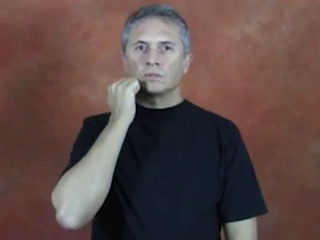
\includegraphics{moskva-end.png}
\caption{\textsc{moscow}}\label{fig:moskva}
}
\end{figure}

None of the individual sign parameters just listed for the
\textsc{moscow} sign above carries lexical semantic information, which
only appears once they are assembled together, and behave like
phonological features in spoken languages. Moreover, substituting one of
them for another can create minimal pairs, just as is the case with
phonological features in spoken languages. To illustrate, changing the
trajectory of the repeated fist movement at the chin on the side of the
dominant hand from straight to clockwise circular changes the sign's
lexical meaning from \textsc{moscow} to \textsc{grandmother}, yet the
movements in question themselves (i.e.~straight \emph{vs.} circular) are
not uniquely associated with the lexical semantics of either
\emph{Moscow} or \emph{grandmother} since they recur in numerous
lexically unrelated signs. Thus, both \textsc{moscow} and
\textsc{grandmother} are arbitrary in the Saussurean sense.

Nevertheless, a significant proportion of sign language vocabulary is
iconic, which makes identifying phonological primitives and even
segments, as well as determining their composition a non-trivial task.
Moreover, scouring the sign language phonology literature creates an
impression that the number of features differentiating one lexical item
from another is virtually limitless, especially when several sign
languages are considered simultaneously, whilst there are surprisingly
few explicit arguments in favour of ascribing those features a
phonological status. On the contrary, the number of minimal pairs
relative to the vast number of features is exceedingly small, which has
to do with the iconic character of certain sublexical elements carrying
semantic information whose status as morphemes is controversial. Indeed,
once these iconic elements are subtracted from a sign, the remaining
residue does not constitute a morpheme either (see van der Kooij 2002
for a detailed discussion of iconicity-related problems for sign
language phonology).

To solve the problem of the overabundance of phonological primitives in
sign language phonologies, van der Kooij (2002) proposes to only use
minimal (or near-minimal) pairs, and treat as phonetic/prosodic residue
those surface realisations that are predictable on the basis of either
the phonological or semantic environment in which they occur.
Anticipating the discussion in Sec.~\ref{sec:data}, the first candidate
for elimination is movement.

In this paper we adopt van der Kooij's (2002) approach of constructing
minimal pairs and augment it by subjecting the preliminarily identified
phonological primitives to statistical testing. In particular, we employ
the Multiple Correspondence Analysis technique with a view to
determining if the primitives in question form natural classes in a
manner roughly similar to the way in which vowels and consonants of
spoken languages form natural classes with a few elements in between.

\hypertarget{sec:data}{%
\section{Data and method}\label{sec:data}}

We take Plaskovitskaya (2018), which is, as far as we are aware, the
only existing description of RSL phonological system to date, as the
point of departure for our study both empirically and analytically. The
data for our study comes from a small annotated corpus presented in
Plaskovitskaya (2018), whose main aim was to test the predictions of
existing approaches to SL phonology against the data from RSL, and to
compile a preliminary inventory of phonological primitives in RSL as
well as sketch a model of their compositional interaction.

\hypertarget{the-model-plaskovitskaya2018}{%
\subsection{The model: Plaskovitskaya
(2018)}\label{the-model-plaskovitskaya2018}}

The model in Plaskovitskaya (2018) is a modified version of Van der
Kooij's (2002) \emph{Dependency model}. Like van der Kooij (2002), and
unlike most of the other models of sign language phonology, it is
inductively organised and crafted on the basis of large datasets, rather
than being deductive in character. It is also hierarchical: head nodes
can restrict the values of their dependent nodes, which, in turn, modify
them. The Dependency model and its descendants differ from most of the
other phonological models (e.g.~ Sandler 1996) in viewing movement as a
phonetic/prosodic reflex rather than as a separate parameter as
described in Sec.~\ref{sec:properties} above. In such a model, signs are
conceptualised as consisting of at least two states (e.g.~an initial
state and a final state), movement being a mere transition from the
initial state to the final state. The proposed hierarchical structure of
an RSL sign is schematically represented in
Fig.~\ref{fig:plaskovitskaya}.

\begin{figure}
\hypertarget{fig:plaskovitskaya}{%
\centering
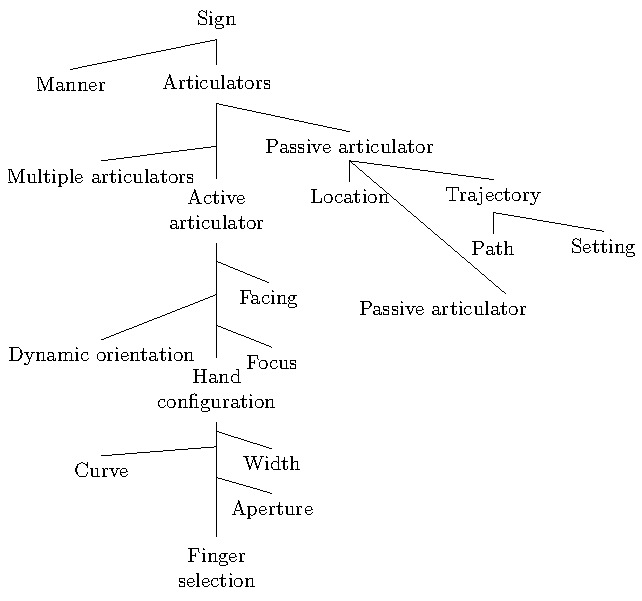
\includegraphics{RSL-phonology-plaskovitskaya-2018-model.pdf}
\caption{segment structure in RSL phonological system (Plaskovitskaya
2018)}\label{fig:plaskovitskaya}
}
\end{figure}

As can be glimpsed from the representation in
Fig.~\ref{fig:plaskovitskaya}, Plaskovitskaya (2018) indeed follows van
der Kooij (2002) in removing movement in the case of the active
articulator from within the purview of phonology and assigns it a
phonetic/prosodic status, whereas the passive articulator is specified
with both Location and Trajectory nodes with an internal complexity of
their own.

By way of illustration, let us consider a minimal working example of the
model at work: the RSL sign for \textsc{betray}, for instance, will
receive the schematic representation in Fig.~\ref{fig:betray}.

\begin{figure}
\hypertarget{fig:betray}{%
\centering
\includegraphics{RSL-phonology-model-BETRAY.pdf}
\caption{\textsc{betray} in Plaskovitskaya (2018)}\label{fig:betray}
}
\end{figure}

The sign involves two articulators: an active articulator (i.e.~the
dominant hand) and a passive articulator corresponding to the middle of
the signer's face (Location: mid-head). Four fingers of the dominant
hand are extended (Curve: straight), and the dominant hand dynamically
changes orientation from prone (i.e.~palm facing down) to neutral.

Perhaps the most significant departure of Plaskovitskaya (2018) from van
der Kooij (2002) concerns the placement of the {[}symmetrical{]} and
{[}crossed{]} features in the hierarchical representation of RSL
signs:\footnote{One set of such difficult cases where annotating the
  citation form of a sign-language verb is insufficient involves the
  so-called \emph{agreeing} verbs (see Pfau, Salzmann \& Steinbach 2018
  for a recent minimalist analysis), also sometimes dubbed
  \emph{indicating} verbs (Schembri, Cormier \& Fenlon 2018), where one
  or more of a sign's parameters can change depending on the presence of
  agreement targets in the sentence.} whilst van der Kooij (2002)
situates them inside the Manner node (which is structurally higher than
any of the articulators), Plaskovitskaya (2018) notes that they are
restricted to the Active Articulator node, and their original
positioning in the Manner node runs the risk of generating unattested
interpretations. To see the necessity of this modification, let us
consider the symmetrical two-handed sign \textsc{deter}, which is
schematically represented in Fig.~\ref{fig:deter}.

The RSL sign for \textsc{deter} involves two active articulators (H1 and
H2) with \textsf{fist} as the requisite handshape synchronically moving
along a straight diagonal path from a higher to a lower position in
front of the passive articulator (trunk). Since both H1 and H2 are
moving symmetrically, the {[}symmetrical{]} feature must be present in
the representation, which van der Kooij (2002) situates in the Manner
node dominating both the active and passive articulators. This makes the
prediction that the sign's symmetricity must also apply to the passive
articulator, contrary to fact. Plaskovitskaya (2018), on the contrary,
introduces an additional node that she dubs Multiple articulators above
the active articulator but crucially below the passive one, thereby
capturing the narrow scope of {[}symmetrical{]} in all cases.

\begin{figure}
\hypertarget{fig:deter}{%
\centering
\includegraphics{RSL-phonology-model-DETER.pdf}
\caption{\textsc{deter} in Plaskovitskaya (2018)}\label{fig:deter}
}
\end{figure}

With the basic familiarity with both the model in hand, we are now in a
position to explore the frequency of occurrence (and cooccurrence) of
the phonetic and phonological features within the RSL lexicon as
compiled by Plaskovitskaya (2018). The motivation behind this is as
follows: since the model ascribes some features (but not others) a
phonological status, this should be visible in the data because subsets
of those features---as well as segments of which they consist---will
form natural classes like vowels do as opposed to consonants in spoken
languages. But first, we offer a few words on the data.

\hypertarget{data}{%
\subsection{Data}\label{data}}

Plaskovitskaya's (2018) corpus consists of 400 primarily monomorphemic,
citation-form verbs taken from the
\href{http://www.spreadthesign.com/be/}{\emph{Spread the Sign}
dictionary} in the Belarusian dialect of RSL. Because the signs normally
appear in the dictionary in their citation form, annotation also
resorted to entries from other dialects of RSL from the same dictionary
as well as field notes from elicitation sessions with the native signers
of the Belarusian dialect of RSL to resolve any potential ambiguities
and facilitate decision making.\footnote{The {[}symmetrical{]} feature
  encodes the identity in handshape between H1 and H2, as well as either
  their identical or mirrored orientation and/or motion. Its semantics
  can be viewed as essentially a copying operation whereby all features
  on the node to which it applies (i.e.~hand configuration and
  orientation) are represented on all articulators in its scope. The
  {[}crossed{]} feature notates the fact that the articulators traverse
  the middle part of the signer's body.}

All entries were manually annotated in ELAN v.5.1 (Crasborn \& Sloetjes
2008). The theoretical model buttressing the annotation is Van der
Kooij's (2002) Dependency model with minor modifications, briefly
addressed directly below. The approach to annotation is intentionally
detailed: even minute features are annotated or introduced to test the
theoretical predictions regarding their status as RSL phonemes, paving
the way for statistically oriented studies such as the one attempted in
this paper. The data, their annotation in the \texttt{.eaf} format and a
dedicated script to facilitate corpus navigation are all freely
available for download as a
\href{https://github.com/ToszaPlaskovickaja/Term_paper}{GitHub
repository} at
\href{https://github.com/ToszaPlaskovickaja/Term_paper}{\texttt{https://github.com/ToszaPlaskovickaja/Term\_paper}}.

Since the model does not view movement as being phonological, some of
the signs will consist of multiple segments. It therefore stands to
reason that whatever procedure is employed for establishing the
restrictions on their occurrence and cooccurrence must deal with those
segments full signs or even syllables.

We first automatically extracted the segments from the annotation and
created a table where all features (19 in total) appear as columns, and
the segments (515 segments in total) as rows. A snapshot of the
resulting table is presented as Fig.~\ref{fig:table}. All data
manipulations were made with R (R Core Team 2018), all visualisations
were created with \texttt{ggplot2} package (Wickham 2016).

\begin{figure}
\hypertarget{fig:table}{%
\centering
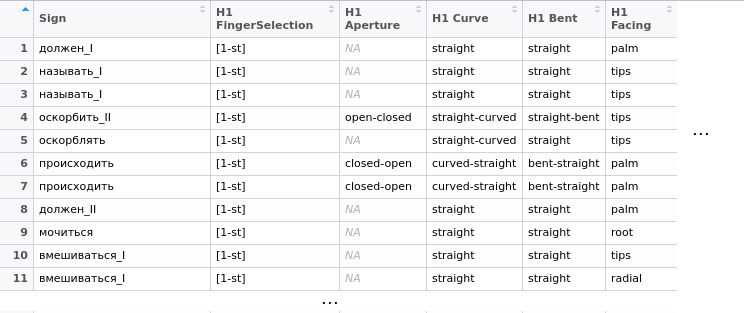
\includegraphics{data-example.png}
\caption{Data structure following automatic extraction of segments from
annotation}\label{fig:table}
}
\end{figure}

In Fig.~\ref{fig:table}, Roman numbers encode distinct lexical items,
and multiple segments forming a single lexical item appear as adjacent
cells in such a way as for their sequential order in the sign to be
reflected: rows 2 and 3, for example, correspond to two segments of one
and the same sign (\textsc{name\_ i}), and the segment in row 2 precedes
the segment in row 3.

\hypertarget{method}{%
\subsection{Method}\label{method}}

To analyse the data that had been collected, we used several tools.
First, we calculated for each feature the ratio of segments employing
one of the feature's values. Simplifying somewhat, we assume here that
the phonological behaviour of a feature could be deduced from the
frequency of occurrence of that feature in an annotated lexicon.

Second, we applied Multiple Correspondence Analysis (MCA, see Husson, Lê
\& Pagès 2017, especially ch.~3). Since all features in Plaskovitskaya's
annotation are instances of categorical data, MCA appears tailor-made to
solve the issue of reducing the dimensionality of the data. In
particular, it provides a way of visualisation both the feature values
and the segments from the annotation in one and the same coordinate
system. Whilst many clusterisation techniques are in principle
compatible with the goals of our study, it is the MCA which allows us to
abstract away from the binary division/union inherently present in
hierarchical clusterisation.

\hypertarget{sec:results}{%
\section{Results}\label{sec:results}}

With regard to the ratio that is plotted on the \(x\) axis in
Fig.~\ref{fig:ratio}, we observe two groups of features plotted on the
\(y\) axis: (i) rare ones (e.g.~H2 Aperture, H2 Focus, H2 Width etc.),
and (ii) the rest (e.g.~Location, H1 Finger Selection etc.). Features
with the lowest ratio seem to be mainly associated with two-handed
features. Amongst the features with the highest frequency rate ratio,
Manner-type features show the lowest rate ratio
(e.g.~manner\_bidirectional), the ratio rising as we move onto the H1
handshape features (e.g.~H1 FingerSelection).

\begin{figure}
\hypertarget{fig:ratio}{%
\centering
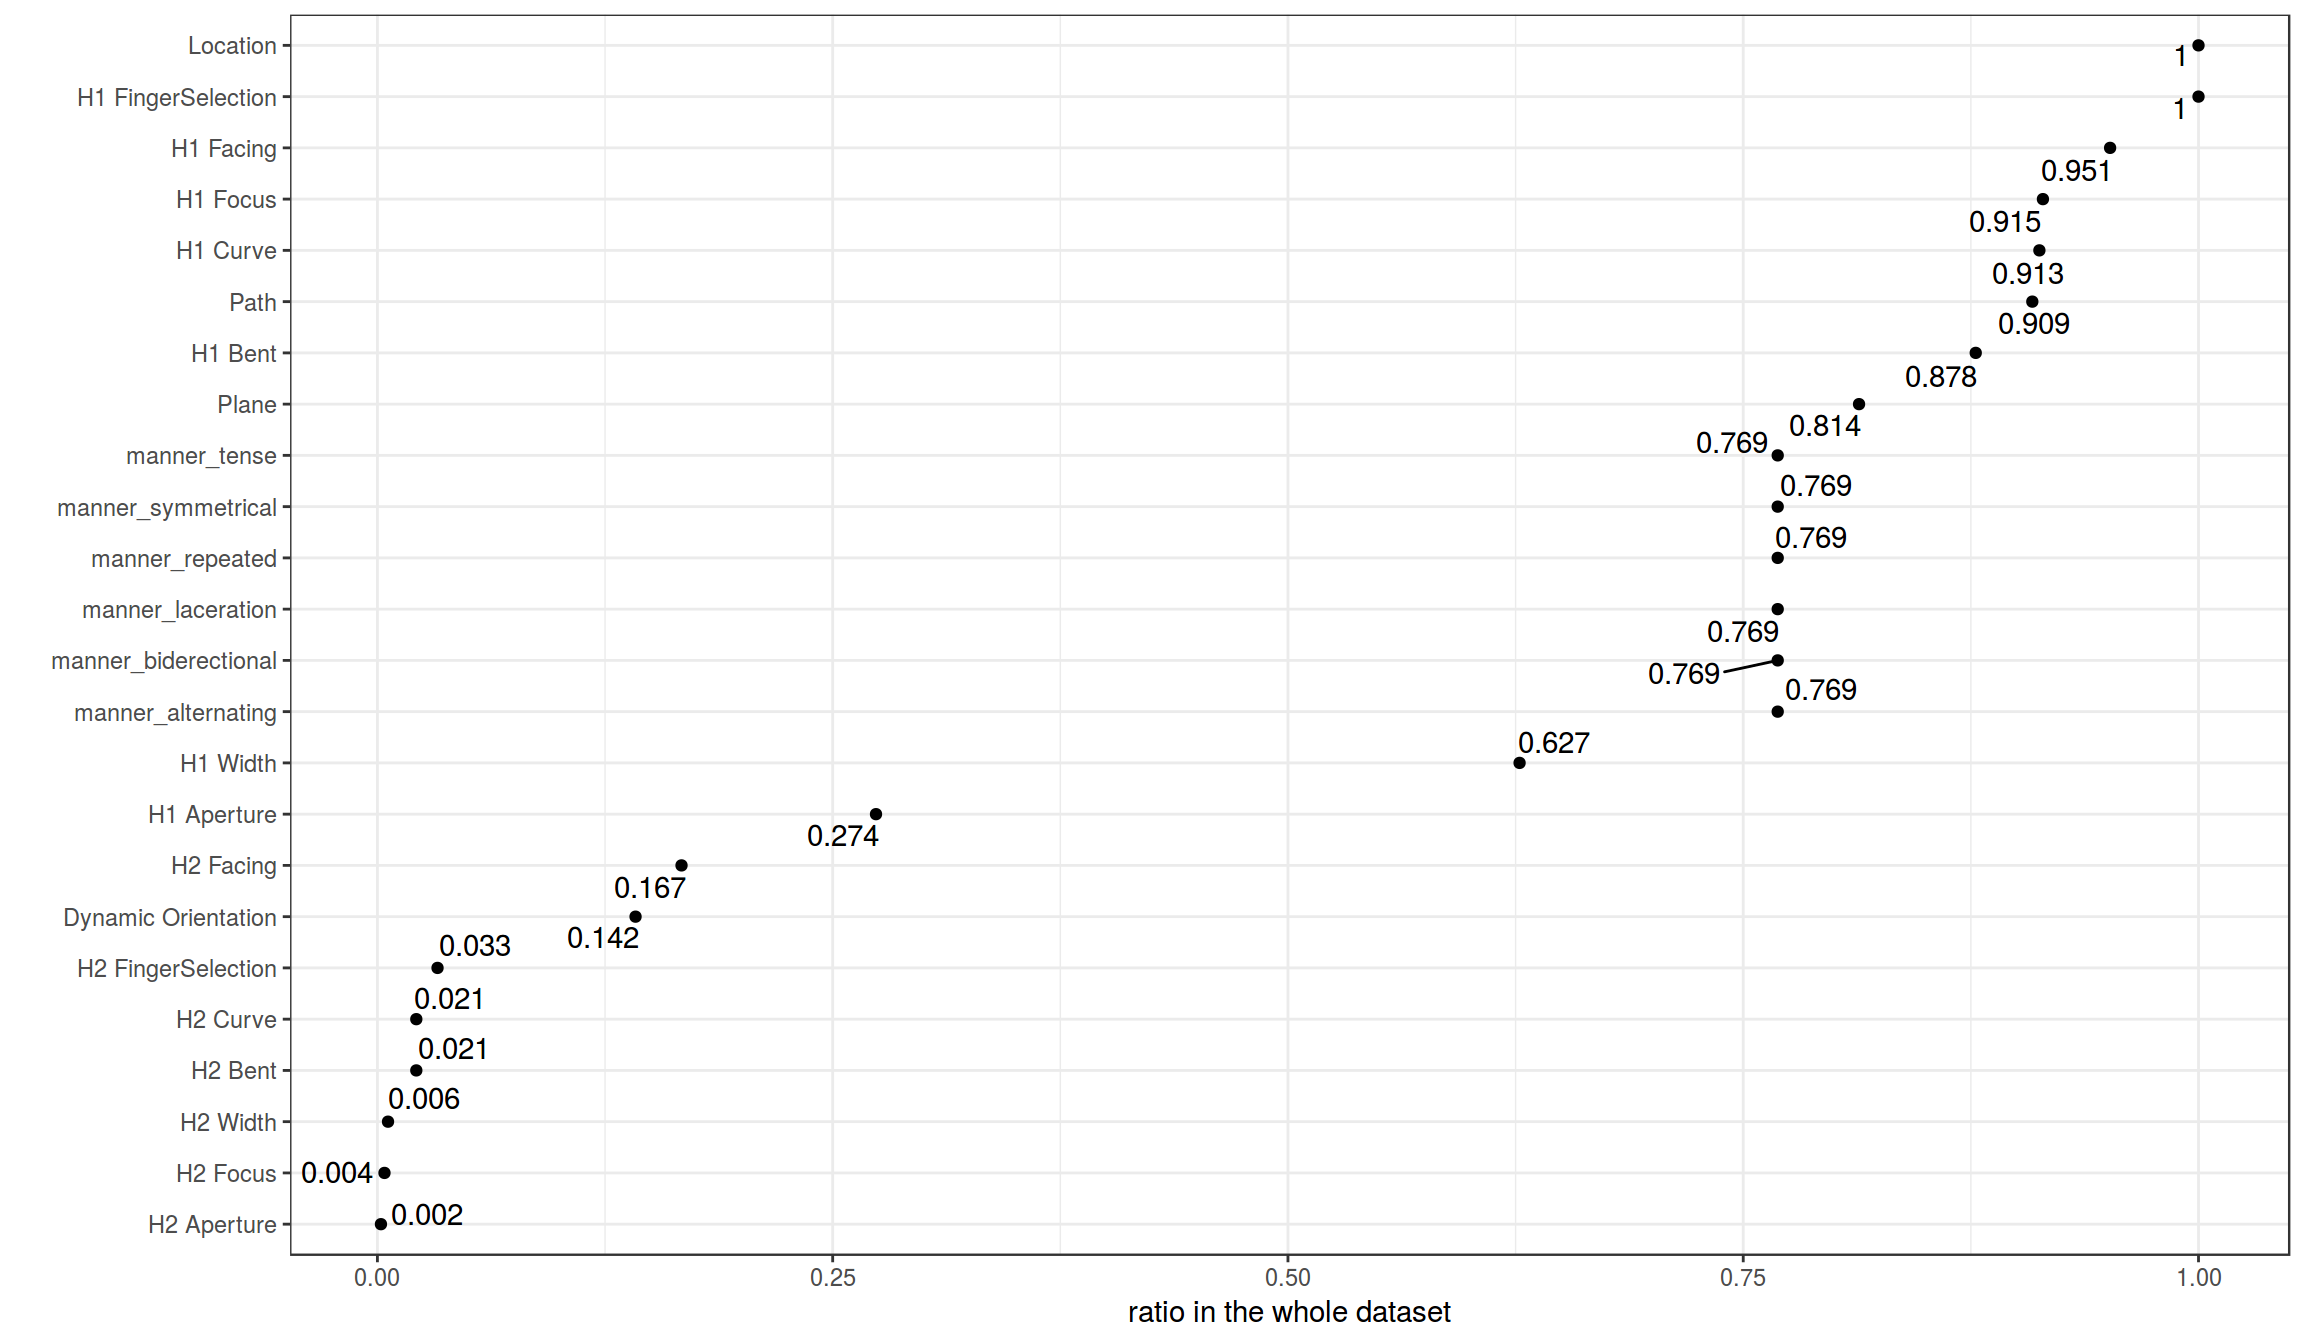
\includegraphics{ratio.png}
\caption{Ratio in the whole dataset}\label{fig:ratio}
}
\end{figure}

Now we turn to the MCA plot in Fig.~\ref{fig:vmeste}. Since MCA provides
dimensionality reduction from multiple dimensions to more optimal
spaces, the \(x\) and \(y\) axes themselves are meaningless. The plot
shows a similar distribution of features. The bottom right-hand corner
of the graph is occupied by features characterising two-handed signs,
which can be explained by those features' low occurrence rate in the
annotation. The second cluster, situated in the top right-hand corner of
the graph, can be loosely characterised as a less marked class
comprising one-handed signs defined by H1 features that include a change
of state from a physiologically less tense state to a physiologically
more tense one.

\begin{figure}
\hypertarget{fig:vmeste}{%
\centering
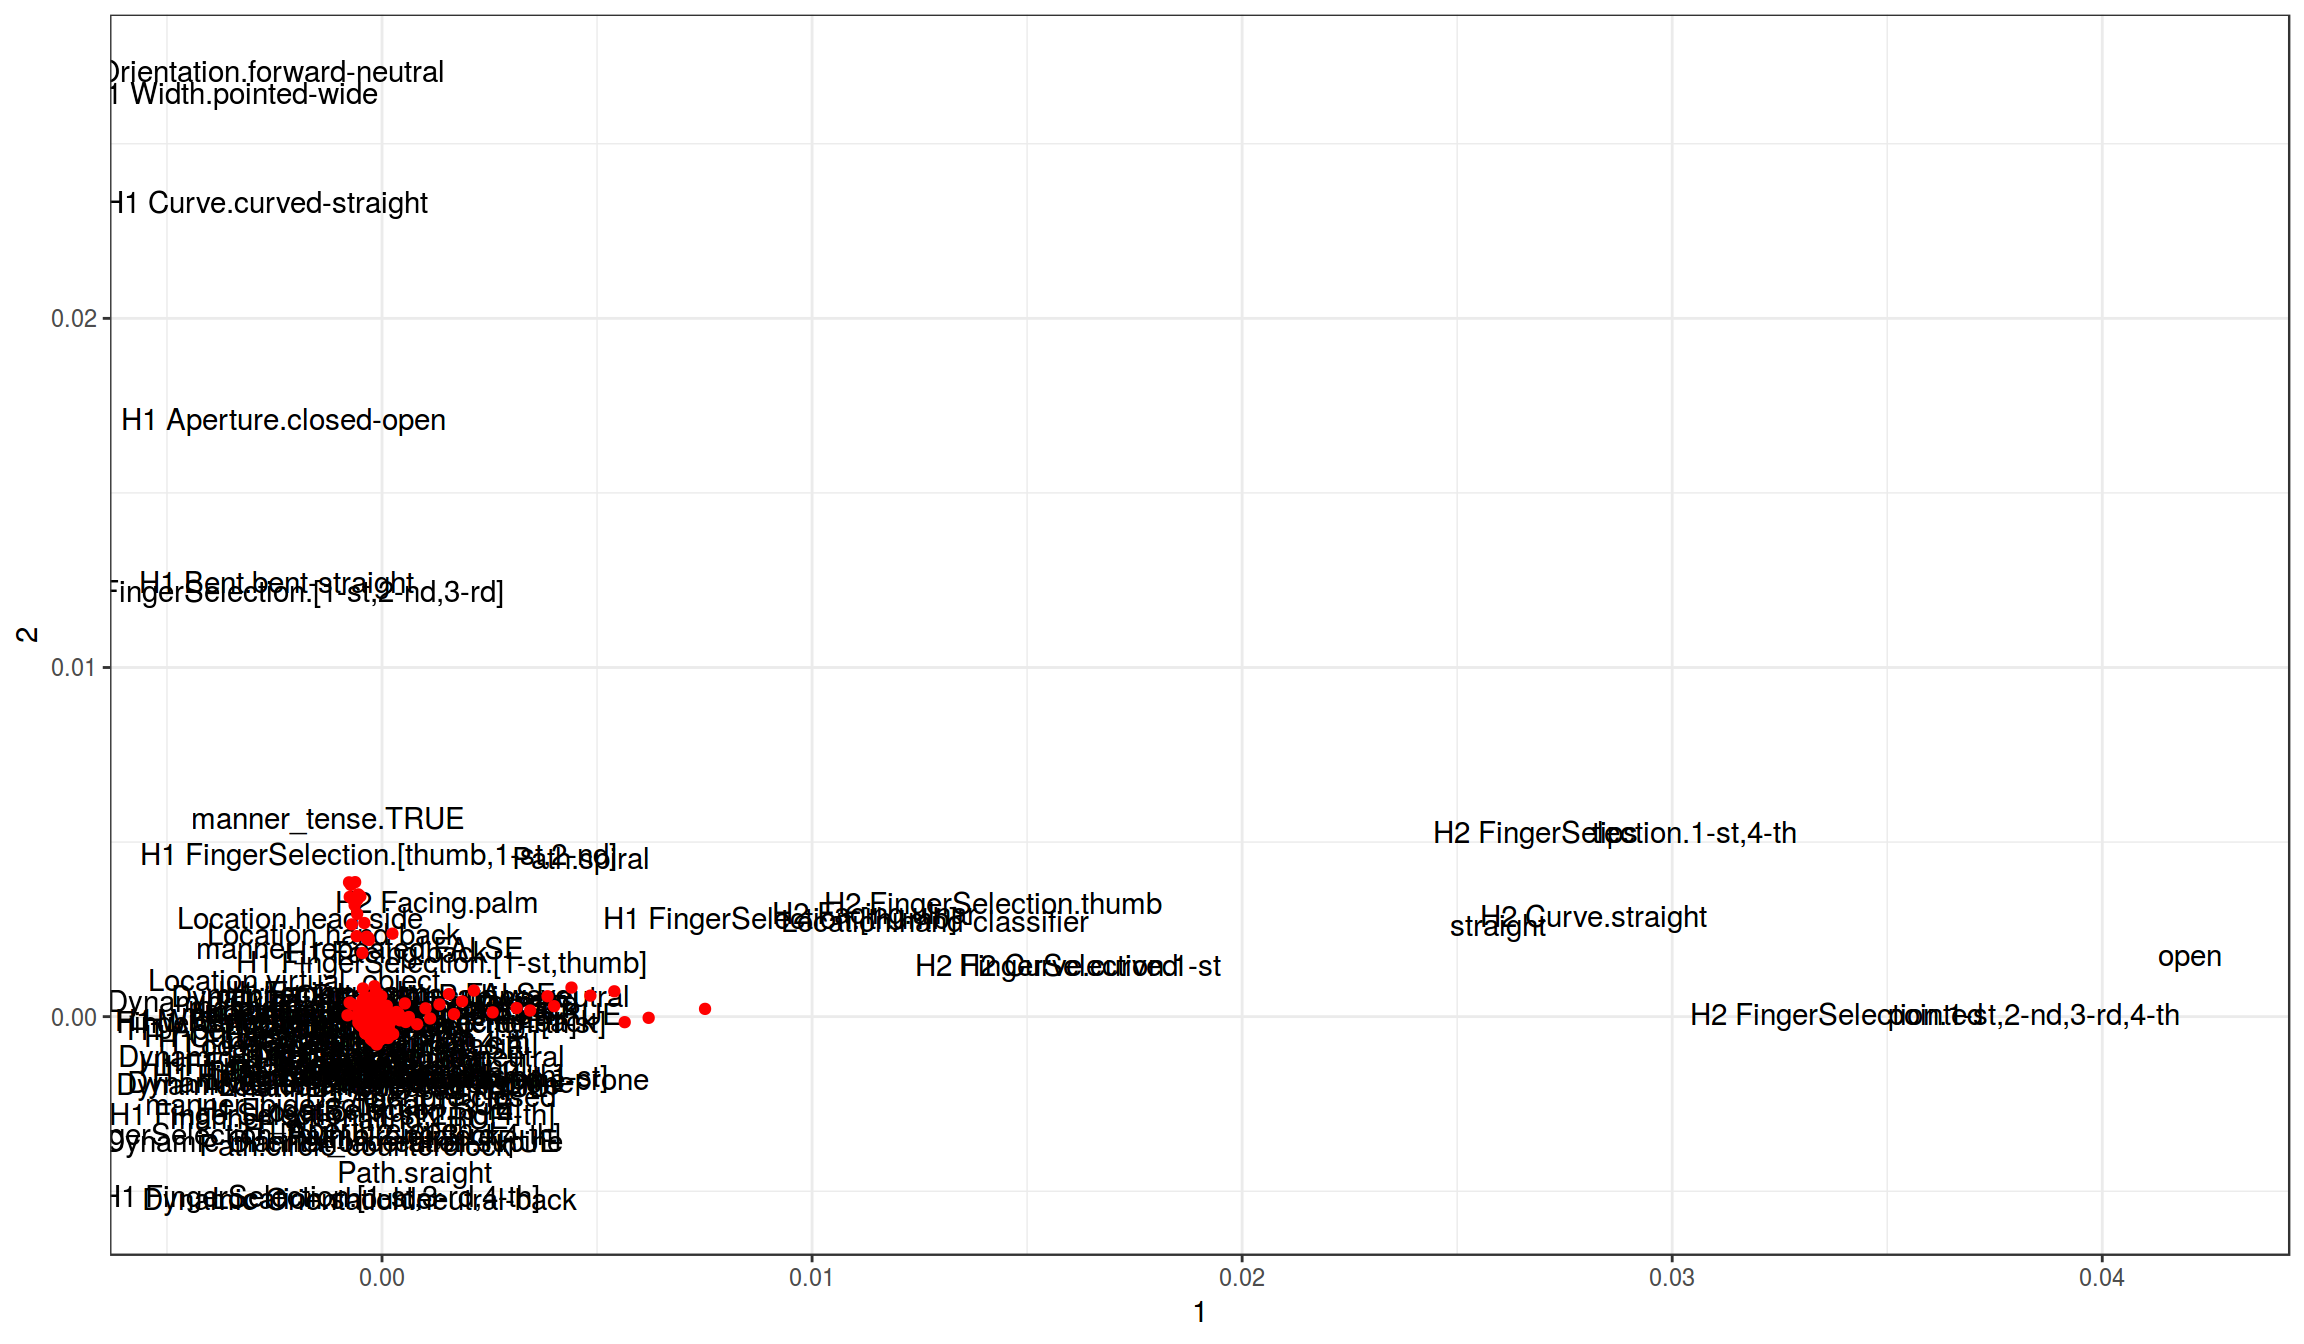
\includegraphics{a-vot-vse-vmeste.png}
\caption{The first two dimensions obtained by MCA for the whole
dataset}\label{fig:vmeste}
}
\end{figure}

To summarise, as a result of applying MCA to our dataset, we discovered
3 clusters corresponding to

\begin{itemize}
\tightlist
\item
  two-handed signs
\item
  signs defined by H1 features including movement to a physiologically
  less tense position
\item
  one-handed signs defined by H1 features including movement to a
  physiologically more tense position.
\end{itemize}

Before proceeding to the discussion of the theoretical significance of
the results obtained in the course of the present study, we address the
issue of iconicity, and the extent to which it can hinder the
identification of phonemes and morphemes of the RSL vocabulary. Since
iconicity is part and parcel of linguistic research into various aspects
of sign languages regardless of theoretical frameworks and persuasions
(see Kimmelman, Klezovich \& Moroz 2018 for a recent discussion and
references), we extended Plaskovitskaya's (2018) annotation scheme to
include iconicity, and fed the resulting annotation back into the MCA,
thereby obtaining the results in Fig.~\ref{fig:iconicity}.

\begin{figure}
\hypertarget{fig:iconicity}{%
\centering
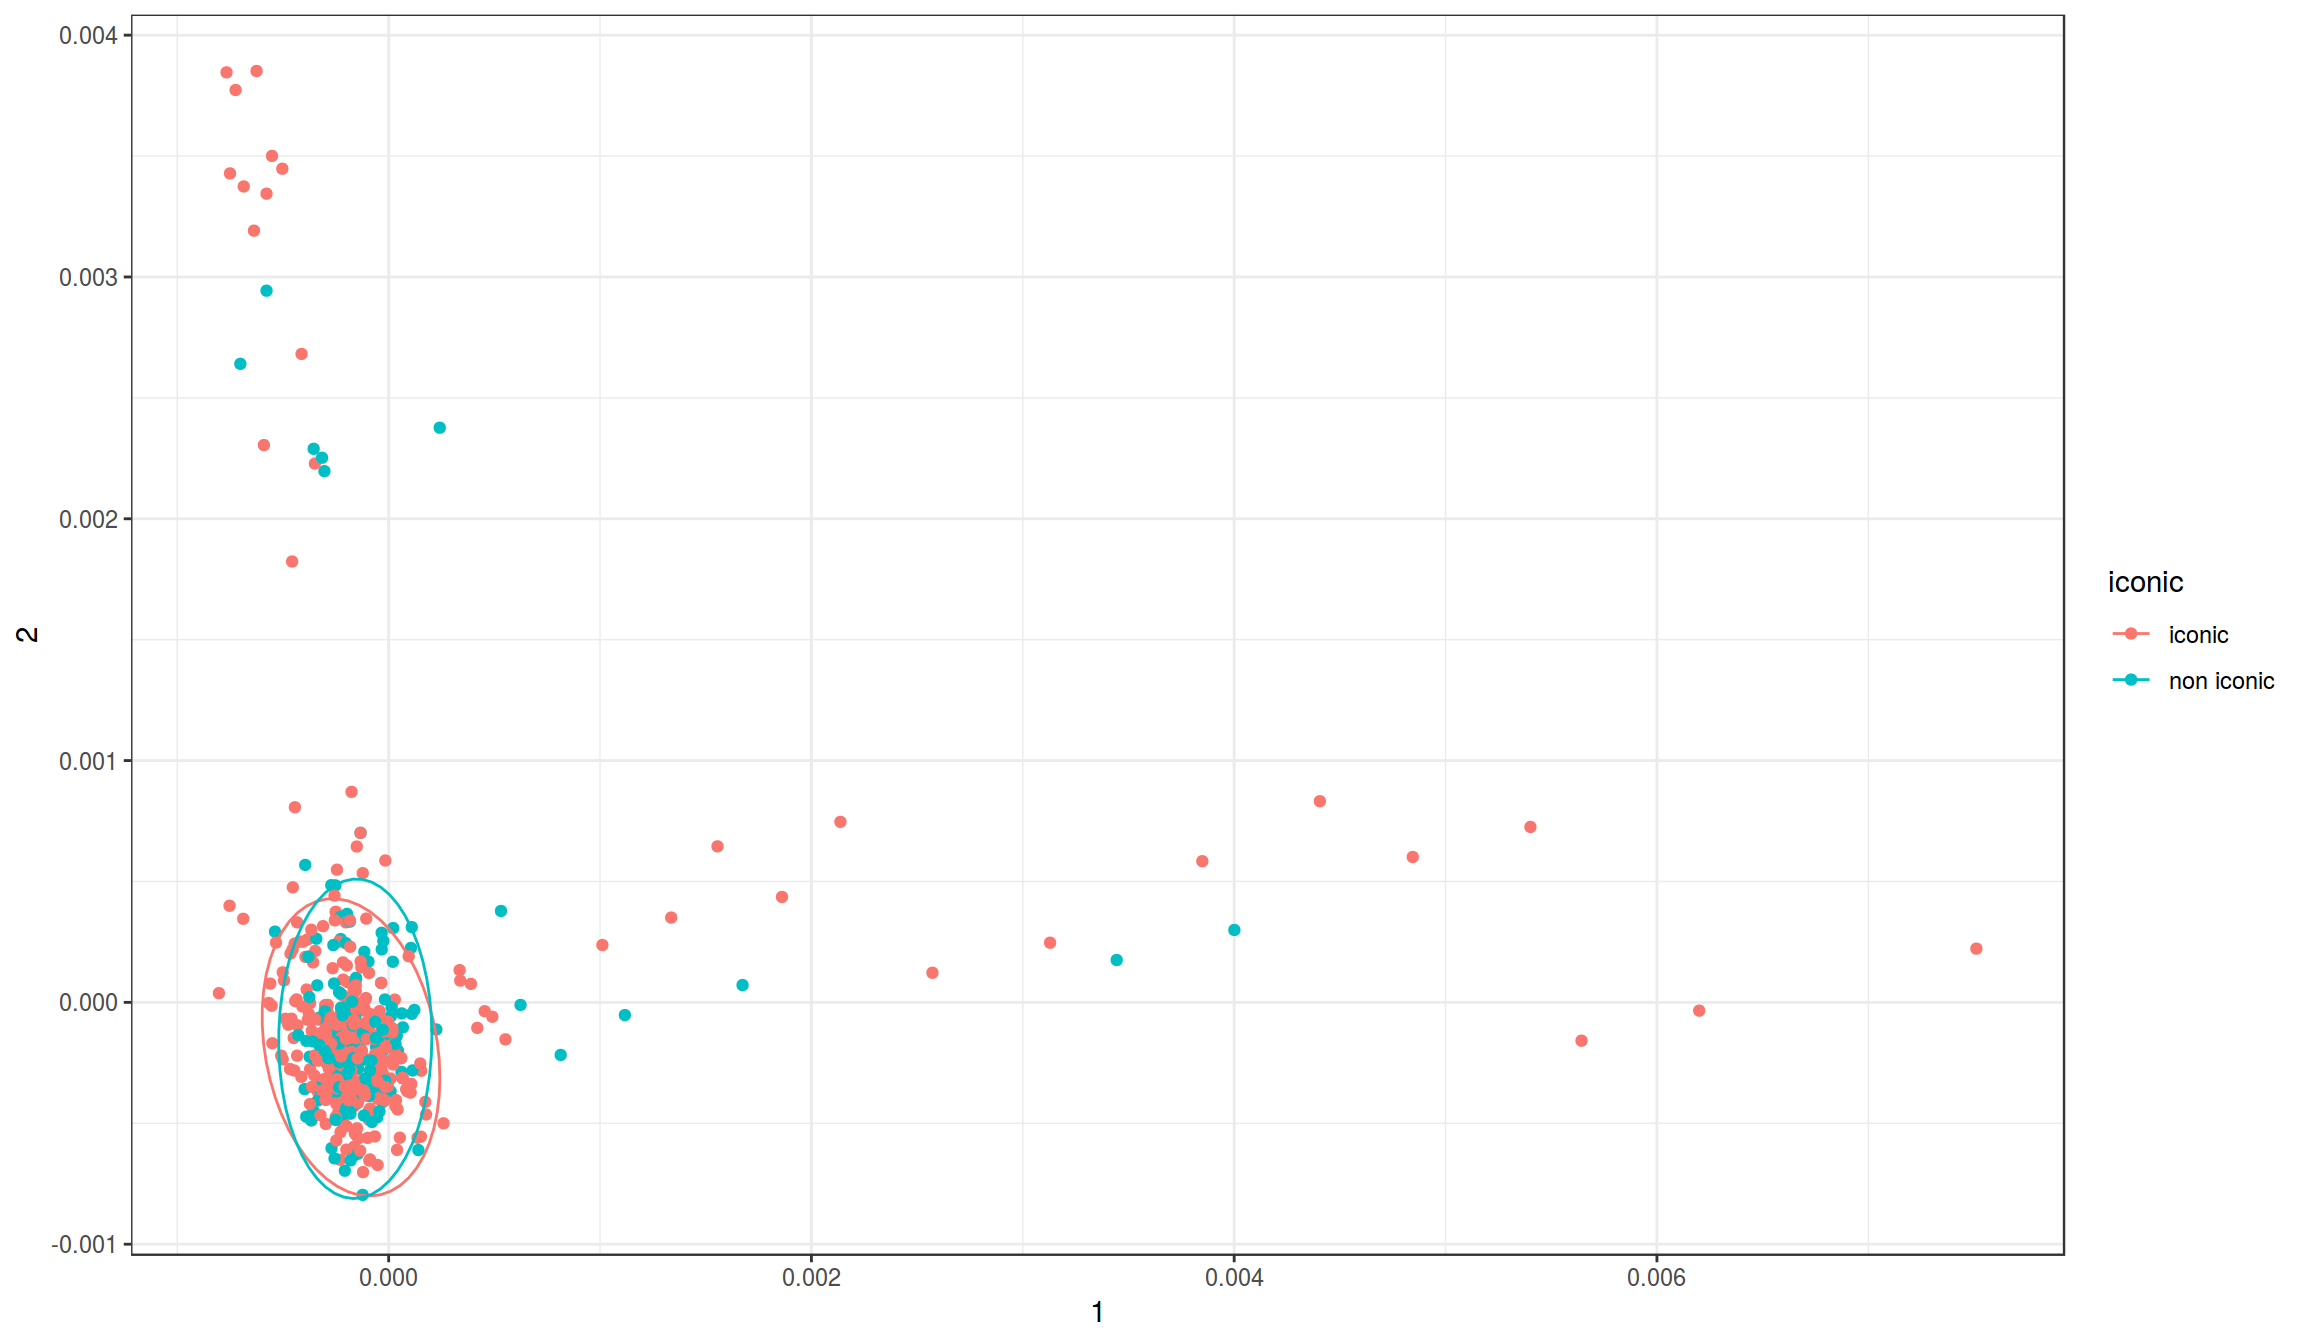
\includegraphics{iconicity.png}
\caption{The first two dimensions obtained by MCA for the whole dataset,
iconicity colour-coded}\label{fig:iconicity}
}
\end{figure}

Fig.~\ref{fig:iconicity} indicates that, on average, iconicity seems not
to correlate with any particular feature from our annotation. We can see
that, even though almost all outliers are iconic, the converse does not
hold: the main cluster involves both iconic and non-iconic signs in
roughly equal proportions.

\hypertarget{sec:discussion}{%
\section{Discussion}\label{sec:discussion}}

In this paper, we have subjected the only existing phonological model of
the structure of RSL signs (Plaskovitskaya 2018) to empirical scrutiny.

The first thing to note concerns the intuitive appeal of clusters
identified by the ratio plot and MCA. Indeed, the distinction between
one-handed and two-handed signs seems important to us as far as sign
languages go, and therefore what stands out in Plaskovitskaya's (2018)
annotation scheme is the lack of consistency in annotating two-handed
signs, which leads to numerous inconsistencies. It is our hope, however,
that the amended annotation will take into consideration two-handed
signs as well as their features, thereby raising their visibility, which
should lead to the features forming a more homogeneous continuum.

What does this tell us about the theory of phonology? We find that a
comparison with spoken languages is useful for illustrating the point at
hand. In spoken language phonology, there is no expectation that all
features should be distributed evenly. Quite to the contrary, situations
abound when an individual feature that is rare nevertheless turns out to
be phonological (e.g.~pharyngealisation in some languages of the
Caucasus), yet this never happens with entire classes of features
(e.g.~features characterising all consonants at the same time).
Therefore, the rare distribution we have observed in the case of so
important a class of features as two-handedness should not have such a
low frequency ratio, which hints at either the sample not being
sufficiently representative or the chosen annotation method being too
inconsistent. Further work will help determine which feature sets play
an important part in RSL phonology, and which natural classes, if any,
can be identified on their basis.

This work also provides a demonstration of a new approach to
investigating the composition of phonological systems. In classic
phonology, all possible oppositions are treated as being equally
significant, and the idea of treating a particular feature within a
given phonological system in a privileged way simply does not arise.
However, just the presence or absence of a phonological feature (that is
common for works on phonological typology) has nothing to say about the
role that feature plays in that system or the feature hierarchies in it.
To take a concrete case, what both Andi (Northeast Caucasian) and French
have in common is the presence of a {[}nasal{]} feature in vowels, yet
this feature is ubiquitous in French whilst being barely present in
Andic. Comparing the importance of phonological features using ratio
plots and MCA is a promising way of revealing non-binary oppositions in
phonological systems of human languages irrespective of modality.

\hypertarget{references}{%
\section*{References}\label{references}}
\addcontentsline{toc}{section}{References}

\hypertarget{refs}{}
\leavevmode\hypertarget{ref-Battison:1974}{}%
Battison, Robbin. 1974. Phonological deletion in American Sign Language.
\emph{Sign language studies} 5(1). Gallaudet University Press. 1--19.

\leavevmode\hypertarget{ref-Boyes:1982}{}%
Boyes-Braem, Penny Kaye. 1982. Features of the Handshape in American
Sign Language.

\leavevmode\hypertarget{ref-Brentari:2011}{}%
Brentari, Diane. 2011. Handshape in sign language phonology.
\emph{Companion to phonology}. 195--222.

\leavevmode\hypertarget{ref-Burkova:2014}{}%
Burkova, Svetlana Igorevna \& Elizaveta Vladimirovna Filimonova. 2014.
Reduplikatsiya v russkom zhestovom yazȳke {[}Reduplication in Russian
Sign Language. \emph{Russkiĭ yazȳk v nauchnom osveschenii}(28).
202--258.

\leavevmode\hypertarget{ref-Burkova:2012}{}%
Burkova, Svetlana Igorevna \& Olga Aleksandrovna Varinova. 2012. K
voprosu o territorial'nom i sotsial'nom var'irovanii russkogo zhestovogo
yazȳka {[}On the matter of territorial and social variation of Russian
Sign Language{]}. ms.

\leavevmode\hypertarget{ref-Channon:2002}{}%
Channon, Rachel. 2002. Signs are single segments: Phonological
representations and temporal sequencing in ASL and other sign languages.
University of Maryland PhD thesis.

\leavevmode\hypertarget{ref-Crasborn:2008}{}%
Crasborn, Onno \& Han Sloetjes. 2008. Enhanced ELAN functionality for
sign language corpora. \emph{Proceedings of the 3rd Workshop on the
Representation and Processing of Sign Languages}. 39--43.

\leavevmode\hypertarget{ref-Emmorey:2008}{}%
Emmorey, Karen, Helsa B. Borinstein, Robin Thompson \& Tamar H. Gollan.
2008. Bimodal bilingualism. \emph{Bilingualism: Language and Cognition}
11(1).
doi:\href{https://doi.org/10.1017/S1366728907003203}{10.1017/S1366728907003203}.

\leavevmode\hypertarget{ref-Fenlon:2018}{}%
Fenlon, Jordan, Kearsy Cormier \& Diane Brentari. 2018. The phonology of
sign languages. In S. J. Hannahs \& Anna R. K. Bosch (eds.), \emph{The
Routledge handbook of phonological theory}, 453--475. London; New York:
Routledge.

\leavevmode\hypertarget{ref-Fontana:2008}{}%
Fontana, Sabina. 2008. Mouth actions as gesture in sign language.
\emph{Gesture} 8(1). John Benjamins. 104--123.

\leavevmode\hypertarget{ref-Husson:2017}{}%
Husson, François, Sébastien Lê \& Jérôme Pagès. 2017. \emph{Exploratory
multivariate analysis by example using R}. CRC Press.

\leavevmode\hypertarget{ref-Israel:2009}{}%
Israel, Assaf \& Wendy Sandler. 2009. Phonological category resolution:
A study of handshapes in younger and older sign languages.
\emph{Cadernos de saude} 2. 13--28.

\leavevmode\hypertarget{ref-Kimmelman:2014}{}%
Kimmelman, Vadim. 2014. Information structure in Russian Sign Language
and Sign Language of the Netherlands. University of Amsterdam
PhD thesis.

\leavevmode\hypertarget{ref-Kimmelman:2018}{}%
Kimmelman, Vadim, Anna Klezovich \& George Moroz. 2018. IPSL: A database
of iconicity patterns in sign languages. Creation and use. In,
\emph{Proceedings of the Eleventh International Conference on Language
Resources and Evaluation (LREC 2018)}.
\url{https://publications.hse.ru/mirror/pubs/share/direct/218828382}.

\leavevmode\hypertarget{ref-Kimmelman:2017}{}%
Kimmelman, Vadim, Maria Kyuseva, Yana Lomakina \& Daria Perova. 2017. On
the notion of metaphor in sign languages: Some observations based on
Russian Sign Language. \emph{Sign Language \& Linguistics} 20(2).
157--182.
doi:\href{https://doi.org/10.1075/sll.00001.kim}{10.1075/sll.00001.kim}.

\leavevmode\hypertarget{ref-Kubucs:2008}{}%
Kubuş, Okan. 2008. An analysis of Turkish Sign Language (TİD) phonology
and morphology. Middle East Technical University PhD thesis.

\leavevmode\hypertarget{ref-Lane:1976}{}%
Lane, Harlan, Penny Boyes-Braem \& Ursula Bellugi. 1976. Preliminaries
to a distinctive feature analysis of handshapes in American Sign
Language. \emph{Cognitive Psychology} 8(2). Elsevier. 263--289.

\leavevmode\hypertarget{ref-Pfau:2008}{}%
Pfau, Roland. 2008. The grammar of headshake: A typological perspective
on German Sign Language negation. \emph{Linguistics in Amsterdam} 1(1).
37--74.

\leavevmode\hypertarget{ref-Pfau:2018}{}%
Pfau, Roland, Martin Salzmann \& Markus Steinbach. 2018. The syntax of
sign language agreement: Common ingredients, but unusual recipe.
\emph{Glossa: A Journal of General Linguistics} 3(1).

\leavevmode\hypertarget{ref-Plaskovitskaya:2018}{}%
Plaskovitskaya, Antonina. 2018. Osnovȳ fonologii russkogo zhestovogo
yazȳka {[}Basics of Russian Sign Language phonology{]}. ms.

\leavevmode\hypertarget{ref-R:2018}{}%
R Core Team. 2018. \emph{R: A language and environment for statistical
computing}. Vienna, Austria: R Foundation for Statistical Computing.
\url{https://www.R-project.org/}.

\leavevmode\hypertarget{ref-Sandler:1989}{}%
Sandler, Wendy. 1989. \emph{Phonological representation of the sign:
Linearity and nonlinearity in American Sign Language}. Dordrecht: Foris.

\leavevmode\hypertarget{ref-Sandler:1996}{}%
Sandler, Wendy. 1996. Phonological features and feature classes: The
case of movements in sign language. \emph{Lingua} 98(1--3). 197--220.
doi:\href{https://doi.org/10.1016/0024-3841(95)00038-0}{10.1016/0024-3841(95)00038-0}.

\leavevmode\hypertarget{ref-Sandier:1999}{}%
Sandler, Wendy. 1999. Cliticization and prosodic words in a sign
language. \emph{Amsterdam Studies in the Theory and History of
Linguistic Science Series 4}. John Benjamins. 223--254.

\leavevmode\hypertarget{ref-Schembri:2018}{}%
Schembri, Adam, Kearsy Cormier \& Jordan Fenlon. 2018. Indicating verbs
as typologically unique constructions: Reconsidering verb `agreement' in
sign languages. \emph{Glossa: A Journal of General Linguistics} 3(1).

\leavevmode\hypertarget{ref-Siedlecki:1993}{}%
Siedlecki Jr, Theodore \& John D Bonvillian. 1993. Location, handshape
\& movement: Young children's acquisition of the formational aspects of
American Sign Language. \emph{Sign Language Studies}. 31--52.

\leavevmode\hypertarget{ref-Stokoe:1960}{}%
Stokoe, William. 1960. \emph{Sign language structure. An outline of the
visual communication systems of the American Deaf}. 1993 reprint. Silver
Spring, MD: Linstok Press.

\leavevmode\hypertarget{ref-vanderKooij:2002}{}%
van der Kooij, Els. 2002. Phonological categories in Sign Language of
the Netherlands: The role of phonetic implementation and iconicity.
Leiden University PhD thesis.

\leavevmode\hypertarget{ref-Wickham:2016}{}%
Wickham, Hadley. 2016. \emph{Ggplot2: Elegant graphics for data
analysis}. Springer-Verlag New York. \url{http://ggplot2.org}.

\leavevmode\hypertarget{ref-Wilbur:1990}{}%
Wilbur, Ronnie B. 1990. Why syllables? What the notion means for ASL
research. \emph{Theoretical issues in sign language research} 1.
University of Chicago Press Chicago, IL. 81--108.
